\documentclass{article}

\usepackage{amsmath}
\usepackage{tikz}
\usetikzlibrary{arrows}

\begin{document}

	Graph nodes table:
	\begin{equation*}
		\begin{aligned}
			& id \quad & coordinates\\
			& 0 \quad & (1,3)\\
			& 1 \quad & (1,1)\\
			& 2 \quad & (2,3)\\
			& 3 \quad & (3,4)\\
			& 4 \quad & (3,1)\\
			& 5 \quad & (4,3)\\
			& 6 \quad & (5,3)\\
			& 7 \quad & (5,1)\\
			& 8 \quad & (7,4)\\
			& 9 \quad & (7,2)\\
		\end{aligned}
	\end{equation*}


	Graph segments table:
	\begin{equation*}
		\begin{aligned}
			& id \quad & start \quad & end \quad & length\\
			& 0 \quad & 0 \quad  & 1 \quad & 2\\
			& 1 \quad & 1 \quad & 4 \quad & 5\\
			& 2 \quad & 0 \quad & 4 \quad & 2\sqrt{2}\\
			& 3 \quad & 0 \quad & 2 \quad & 1\\
			& 4 \quad & 2 \quad & 3 \quad & \sqrt{2}\\
			& 5 \quad & 4 \quad & 3 \quad & 3\\
			& 6 \quad & 3 \quad & 5 \quad & \sqrt{2}\\
			& 7 \quad & 4 \quad & 5 \quad & \sqrt{5}\\
			& 8 \quad & 5 \quad & 7 \quad & \sqrt{5}\\
			& 9 \quad & 5 \quad & 6 \quad & 1\\
			& 10 \quad & 6 \quad & 7 \quad & 2\\
			& 11 \quad & 6 \quad & 8 \quad & \sqrt{5}\\
			& 12 \quad & 7 \quad & 9 \quad & \sqrt{5}\\
			& 13 \quad & 9 \quad & 8 \quad & 2\\
		\end{aligned}
	\end{equation*}


	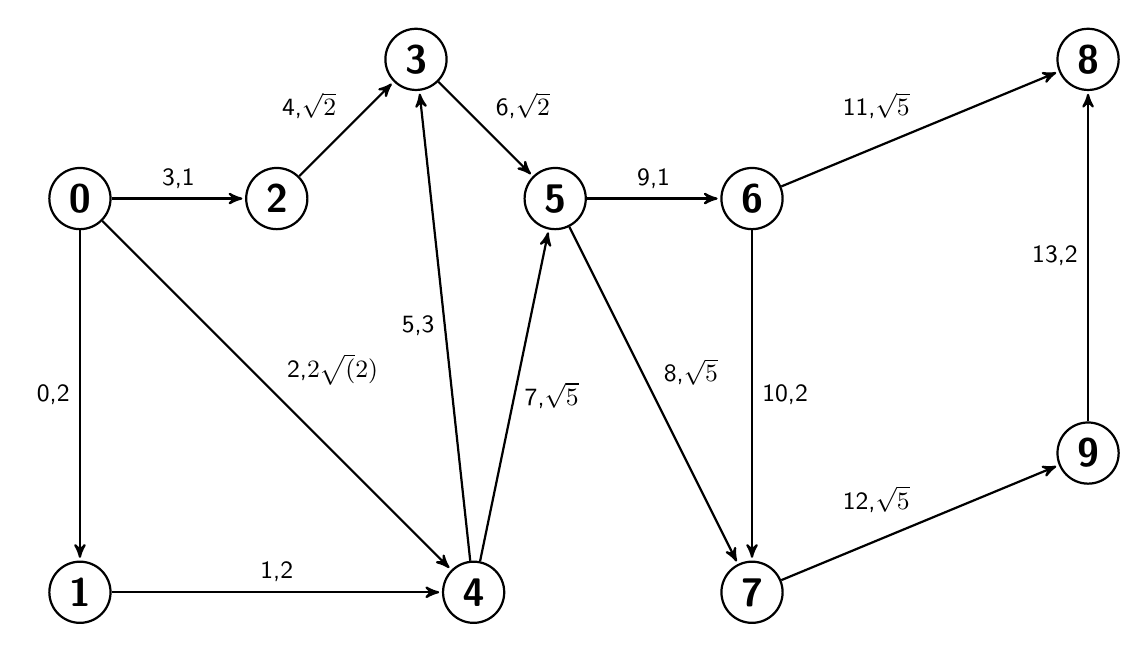
\begin{tikzpicture}[->,>=stealth',shorten >=1pt,auto,node distance=2.5cm,
	  thick,main node/.style={circle,fill=white!20,draw,font=\sffamily\Large\bfseries}]

		\node[main node] (0) {0};
		\node[main node] (90) [below of=0, draw=none]{};
		\node[main node] (1) [below of=90] {1};
		\node[main node] (2) [right of=0] {2};
		\node[main node] (3) [above right of=2] {3};
		\node[main node] (91) [right of=1, draw=none] {};
		\node[main node] (4) [right of=91] {4};
		\node[main node] (5) [below right of=3] {5};
		\node[main node] (6) [right of=5] {6};
		\node[main node] (96) [below of=6, draw=none] {};
		\node[main node] (7) [below of=96] {7};
		\node[main node] (97) [right of=7, draw=none] {};
		\node[main node] (9) [above right of=97] {9};
		\node[main node] (98) [above of=9, draw=none] {};
		\node[main node] (8) [above of=98] {8};

	\path[every node/.style={font=\sffamily\small}]
		(0) edge node [left] {0,2} (1)
			edge node [above] {3,1} (2)
			edge node {2,$2\sqrt(2)$} (4)
		(1) edge node [above] {1,2} (4)
		(2) edge node {4,$\sqrt{2}$} (3)
		(3) edge node {6,$\sqrt{2}$} (5)
		(4) edge node [left] {5,3} (3)
			edge node [right] {7,$\sqrt{5}$} (5)
		(5) edge node [above] {9,1} (6)
			edge node {8,$\sqrt{5}$} (7)
		(6) edge node [right] {10,2} (7)
			edge node {11,$\sqrt{5}$} (8)
		(7) edge node {12,$\sqrt{5}$} (9)
		(9) edge node {13,2} (8);		

	\end{tikzpicture}


\end{document}
